\scanpage{21}
\deleted{\unsure{Le} \illegible{2} \unsure{donne}} \deleted{\inserted{Considérons le diagramme}}

\diagram{\begin{tikzcd}[ampersand replacement=\&,column sep=small]
\deleted{0}\arrow[r,dash] \& \deleted{\mathrm{Hom}(B,A')}\arrow[r,dash]\arrow[d] \& \deleted{\mathrm{Hom}(B,A)}\arrow[r,dash]\arrow[d] \& \deleted{\mathrm{Hom}(B,A'')}\arrow[r] \& \deleted{0}\\
\deleted{0}\arrow[r,dash] \& \deleted{\mathrm{Hom}(SB,SA')}\arrow[r] \& \deleted{\mathrm{Hom}(SB,SA)}\arrow[r,dash] \& \deleted{\mathrm{Hom}(\unsure{SB|B},SA'')}\arrow[r] \& \deleted{0}
\end{tikzcd}}

\deleted{alors les deux flèches verticales et la \unsure{deuxième|dernière} horizontale sont injectives, donc aussi la première horizontale, donc $B'\unsure{-|\to}B$ est injectif. En prenant $\mathrm{Hom}(S,B)$, on voit de $=$ que $B-B''$ est surjectif, d'autre part $S$ étant injectif, le composé $B'\to B\to B''$ \deleted{\unsure{est}} est nul.}

$vu=0$, et on aura $S(\mathrm{Ker}\,v/\mathrm{Im}\,u)=\mathrm{Ker}\,S(v)/\mathrm{Im}(Su)$ et le \deleted{\unsure{de|des}} premier \unsure{mb} est nul si et seulement si $\mathrm{Ker}\,v/\mathrm{Im}\,u$ l'est, on voit que $\Sigma$ est une suite exacte si et seulement si $S$ l'est.

\figure{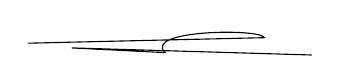
\begin{tikzpicture}[x=1cm,y=1cm]\draw (0,.10)--(3,.17).. controls (2.95,.29) and (1.45,.27) .. (1.74,-.02)--(.55,.04)--(3.6,-.05);\end{tikzpicture}}

Nous avons maintenant ce qu'il faut [catégorie de ``suites exactes'' $\Longleftrightarrow$ catégorie d'``injectifs''] pour faire une théorie ``relative'' des foncteurs dérivés $\mathcal C\to\mathcal D$, où $\mathcal D$ est une véritable catégorie \uline{abélienne}. De plus, \inserted{une} \deleted{\unsure{l'}}itération des foncteurs $TS=C^0$ :

\[
C^1(A)=C^0(A)/\mathrm{Im}\,A\qquad C^i(A)=C^0(C^{i-1}(A)/\mathrm{Im}(C^{\deleted{\unsure{i}}i-2}(A)))\quad\text{si }i\geq2 .
\]

donne une résolution \inserted{$S$-injective} \uline{canonique} (fonctorielle) de $A\in\mathcal C$

% archive sheet number: 20
